\section{迭代求解器的预条件子}\label{sec:chapter9-preconditioners}

\begin{note}[预条件子]
\label{note:chapter9-preconditioners}
众所周知,采用预条件子可以显著改善迭代求解器的性能.预条件子是对 $\mathcal A^{-1}$ 的近似,且能够以相对较低的计算代价求得.这种近似可以是一个固定矩阵、一种数值(迭代)方法,或二者的组合.

预条件分为左预条件和右预条件.记预条件子为 $M^{-1}$.对于左预条件,迭代求解器求解的系统由式\hyperref[eq:chapter9-coupled-system]{(9.1)}改为
\[
 M^{-1}\mathcal A\bm x=M^{-1}\bm y.
\]
采用右预条件时,迭代求解器求解
\[
 \mathcal A M^{-1}\bm z=\bm y,
 \qquad \bm x=M^{-1}\bm z.
\]
同一迭代求解器配合同一预条件子,采用左预条件和右预条件时的表现可能不同.例如,左、右预条件 GMRES 最小化的残量不同;详见\textcite[第 9.3.4 节]{Saad2003}.
\end{note}



\subsection{不完全分解}\label{subsec:chapter9-incomplete-factorizations}

\begin{note}[不完全分解]
\label{note:chapter9-incomplete-factorizations}
对稀疏矩阵 $\mathcal A$ 作 LU 分解时,所得因子 $L$ 和 $U$ 通常会比 $\mathcal A$ 稠密得多.在不完全 LU 分解(incomplete LU factorization,ILU)中,$L$ 和 $U$ 保留与 $\mathcal A$ 相同的稀疏结构:$L$ 的稀疏结构对应于 $\mathcal A$ 的严格下三角部分,$U$ 的稀疏结构对应于 $\mathcal A$ 的上三角部分.执行不带主元选取的标准 LU 分解算法时,舍弃所有不符合预定稀疏结构的项,由此得到不完全分解
\begin{equation}\label{eq:chapter9-ilu-incomplete-factorization}
 \mathcal A=LU+E,
\end{equation}
其中 $E$ 为误差矩阵.

例如,\textcite{DahlWille1992}指出,对 $\mathcal A$ 作 ILU 分解时不采用主元选取,并不一定会导致算法失败.首先,应按压力自由度排在最后的方式排列自由度,这与式\hyperref[eq:chapter9-coupled-system]{(9.1)}中的排列一致.其次,需要给定稀疏矩阵 $C$,其稀疏结构应包含压力自由度之间的全部连接(与 inf-sup 稳定化方法中的情形相同),并将 $C$ 的所有项初始化为零.在这两个条件下,\textcite{DahlWille1992}观察到,不完全分解过程中主对角线上的零项会消失,因此不会发生除以零.

所谓 ILUT$(l,\tau)$ 方法(\textcite[第 10.4.1 节]{Saad2003})允许保留 LU 分解中模大于阈值 $\tau\ge0$ 的项,即使这些项不符合原有稀疏结构.对于当前行,只保留 $L$ 部分中按绝对值计最大的 $l$ 项、$U$ 部分中按绝对值计最大的 $l$ 项,另加对角项.这样得到式\hyperref[eq:chapter9-ilu-incomplete-factorization]{(9.2)}形式的不完全分解;其误差矩阵的非零项预计会更小,同时避免完整 LU 分解产生的全部填充.
\end{note}

\begin{note}[带填充的不完全 LU 预条件子]
\label{note:chapter9-ilu-fill-in}
\textcite{Konshin2015}提出了一种 ILU 预条件子,用于求解非定常 Navier--Stokes 方程组离散后产生的线性鞍点问题.该预条件子对整体矩阵 $\mathcal A$ 作不带主元选取的分解,其形式为
\[
 \mathcal A=LU+L R_u+R_l U+E,
\]
其中 $R_u$ 为严格上三角矩阵,$R_l$ 为严格下三角矩阵,$E$ 仍为误差矩阵.给定两个参数 $\tau_1\ge\tau_2>0$,构造分解时要求 $L$ 和 $U$ 的非对角项要么为零,要么其绝对值大于 $\tau_1$;而 $R_u$ 和 $R_l$ 的非对角项要么为零,要么其绝对值属于 $(\tau_2,\tau_1]$.因此,误差矩阵 $E$ 中的项为 $O(\tau_2)$.如\textcite{Konshin2015}所述,该方法的填充量由 $\tau_1$ 决定;当 $\tau_2=O(\tau_1)$ 时,所得预条件子的质量则由 $\tau_2$ 控制.

要使该预条件子高效工作,首先需要对矩阵 $\mathcal A$ 进行适当缩放.\textcite{Konshin2015}表明,选取合适的 $\tau_1$ 和 $\tau_2$ 后,该预条件子可用于一大类黏度下的层流三维非定常 Navier--Stokes 问题,并能高效求解.
\end{note}

\index{预条件子!左预条件}
\index{预条件子!右预条件}
\index{不完全 LU 分解(ILU)}
\index{不完全 LU 预条件子!带填充}

\subsection{耦合多重网格方法}
\label{subsec:chapter9-coupled-multigrid}\label{subsec:multigrid-method}
\label{subsec:chapter9-iterative-solvers}

\begin{note}[多重网格方法]
\label{note:chapter9-multigrid-methods}\label{note:multigrid-method}
多重网格方法通过一系列网格层级求解线性方程组.在每一层上,都近似求解相应的方程;只有在最粗层(称为第 0 层)上,方程才可能被高精度求解.多重网格方法需要在相邻层级之间传递信息:由细层向粗层传递称为限制,由粗层向细层传递称为延拓.关于多重网格方法的介绍可参见\textcite{Hackbusch1985,Trottenberg2001,Briggs2000}.

下面介绍用于求解式\hyperref[eq:chapter9-coupled-system]{(9.1)}的多重网格方法的组成部分.该方法同时求解速度 $\bm u$ 和压力 $p$ 两类未知量,因而称为耦合多重网格方法.它由以下部分定义:
\begin{itemize}
  \item 网格层级,见笔记\hyperref[note:chapter9-grid-hierarchy]{9.12};
  \item 粗层系统矩阵的定义,见笔记\hyperref[note:chapter9-coarse-system-matrices]{9.13};
  \item 网格间传递算子:
  \begin{itemize}
    \item 函数延拓,见笔记\hyperref[note:chapter9-function-prolongation]{9.14};
    \item 缺陷限制,见笔记\hyperref[note:chapter9-defect-restriction]{9.18};
    \item 函数限制,见笔记\hyperref[note:chapter9-function-restriction]{9.19};
  \end{itemize}
  \item 细层上的光滑子,见笔记\hyperref[note:chapter9-vanka-smoother]{9.20};
  \item 粗网格求解器,见笔记\hyperref[note:chapter9-coarse-grid-solver]{9.24}.
\end{itemize}
\end{note}

\index{多重网格方法}


\begin{note}[网格层级]
\label{note:chapter9-grid-hierarchy}
定义多重网格层级有多种方式.标准做法是沿用几何网格的层级,并在各层上采用相同的离散方法.不过,多重网格层级也可以多于几何网格层级,并且粗层可采用不同于最细层的离散方法.图\hyperref[fig:chapter9-multigrid-approaches]{9.1}所示的多重离散多层方法就是一例.

\begin{elegantfigure}[333.25pt]
\includegraphics[page=663,pagebox=cropbox,trim=53.00bp 464.15bp 53.11bp 61.50bp,clip,width=333.25pt]{../input/source/Finite Element Methods for Incompressible Flow Problems.pdf}
\captionof{figure}{标准多重网格方法(左)与面向高阶离散的多重离散多层方法(右).}
\label{fig:chapter9-multigrid-approaches}
\end{elegantfigure}

在\textcite{JohnMatthies2001}关于例题\hyperref[ex:appendix-d-5]{D.5}以及\textcite{John2002}关于例题\hyperref[ex:appendix-d-6]{D.6}的数值研究中,研究者发现:对于某些高阶有限元离散所得的线性鞍点问题,标准多重网格方法会遇到困难.高阶有限元离散能够较准确地计算感兴趣量,参见例题\hyperref[ex:steady-ns-flow-around-cylinder]{6.36}.与此相反,带迎风稳定化的最低阶非协调离散的精度较低,参见笔记\hyperref[note:oseen-upwind-nonconforming]{5.58};但标准多重网格方法已被证明是一种效率很高的求解器,另见\textcite{JohnTobiska2000}.由此产生了一个构造高阶有限元离散多层方法的思路:以稳定的最低阶非协调有限元离散所用的多层方法为基础.这就是图\hyperref[fig:chapter9-multigrid-approaches]{9.1}所示的多重离散多层方法.

该方法的多层层级比几何网格层级多一层.在最细的几何网格(第 $L$ 层)上采用两种离散方法:其中一种是所关注的高阶离散,它构成多层层级的最细层;另一种是在几何第 $L$ 层上采用带迎风稳定化的最低阶非协调离散.在所有更粗的几何层上,也采用经过稳定化的最低阶非协调离散.

在多重网格方法中,网格序列的组织方式称为循环.最常见的多重网格循环见图\hyperref[fig:chapter9-multigrid-cycles]{9.2}.

\begin{elegantfigure}[333.25pt]
\includegraphics[page=664,pagebox=cropbox,trim=53.00bp 416.15bp 53.11bp 61.00bp,clip,width=333.25pt]{../input/source/Finite Element Methods for Incompressible Flow Problems.pdf}
\captionof{figure}{多重网格 V 循环、F 循环和 W 循环(依次为左上、右上和下图);$s$ 表示光滑,$r$ 表示限制,$p$ 表示延拓,$e$ 表示精确求解器.}
\label{fig:chapter9-multigrid-cycles}
\end{elegantfigure}
从浮点运算次数看,V 循环代价最低,W 循环代价最高;从稳定性看,情况正好相反.F 循环通常是在计算代价与稳定性之间折中的一种选择.
\end{note}

\index{多重网格方法!V 循环}
\index{多重网格方法!F 循环}
\index{多重网格方法!W 循环}
\index{多层方法!多重离散}


\begin{note}[粗层线性系统的定义]
\label{note:chapter9-coarse-system-matrices}
所谓 Galerkin 投影利用第 $l$ 层的系统矩阵以及延拓、限制算子,定义第 $l-1$ 层的系统矩阵.然而,这种方法无法在不同层级上使用不同的离散方法,而后者正是多重离散多层方法的核心思想.此外,从实现角度看,在粗层上直接组装系统矩阵、并采用与最细层相同的组装方式,似乎更为简便.因此,实际中常采用直接组装.
\end{note}

\begin{note}[函数延拓]
\label{note:chapter9-function-prolongation}
多重网格方法需要将有限元函数从某一层级传递到紧邻的更细层.在多重离散多层方法中,相邻层上的有限元空间可能并不嵌套,因此传递算子必须能够处理这种情形.\textcite{Schieweck2000}提出并分析了一种可在几乎任意有限元空间之间传递函数的算子.下面以标量有限元函数为例,较详细地介绍这一算子.它基于节点泛函的概念(见笔记\hyperref[note:appendix-b-18]{B.18})和局部基(见笔记\hyperref[note:appendix-b-20]{B.20}).

考虑从有限元空间 $V_{l-1}^h$ 到有限元空间 $V_l^h$ 的传递(延拓).设 $\mathcal T_{l-1}$ 和 $\mathcal T_l$ 分别为相应的区域剖分,其中 $\mathcal T_l$ 由 $\mathcal T_{l-1}$ 加密得到,或者 $\mathcal T_l=\mathcal T_{l-1}$.后一种情形适用于多重离散多层方法中的 $l=L+1$,见图\hyperref[fig:chapter9-multigrid-approaches]{9.1}.

设 $S_l^h$ 是定义在 $\mathcal T_l$ 上的不连续有限元空间:
\[
 S_l^h=\left\{w\in L^2(\Omega):
     w|_K\in S_l^h(K)\quad\forall K\in\mathcal T_l\right\}.
\]
局部空间 $S_l^h(K)$ 的选取取决于 $V_{l-1}^h$ 和 $V_l^h$,并须满足包含关系
\begin{equation}\label{eq:chapter9-transfer-space-inclusion}
 V_{l-1}^h+V_l^h\subseteq S_l^h.
\end{equation}
从实际实现角度看,构造传递算子时并不需要用到局部空间 $S_l^h(K)$.从理论角度看,可以证明,对于由单形构成的剖分,总能找到适当的 $S_l^h(K)$,见\textcite{JohnKnoblochMatthiesTobiska2002}.

利用整体节点泛函(见笔记\hyperref[note:appendix-b-23]{B.23}),延拓传递算子定义为
\begin{equation}\label{eq:chapter9-function-prolongation}
 P_{l-1}^{l}:S_l^h\longrightarrow V_l^h,
 \qquad
 P_{l-1}^{l}w=\sum_{i=1}^{\dim(V_l^h)}N_{l,i}(w)\,\varphi_{l,i}^h,
\end{equation}
其中 $\{\varphi_{l,i}^h\}_{i=1}^{\dim(V_l^h)}$ 是 $V_l^h$ 的有限元基,$N_{l,i}$ 是第 $l$ 层的整体节点泛函,满足
\[
 N_{l,i}(\varphi_{l,j}^h)=\delta_{ij}.
\]
由包含关系\hyperref[eq:chapter9-transfer-space-inclusion]{(9.3)}可知,算子\hyperref[eq:chapter9-function-prolongation]{(9.4)}特别适用于 $V_{l-1}^h$ 中的函数.
\end{note}

\begin{note}[用局部泛函计算整体泛函]
\label{note:chapter9-local-functionals}
设 $\{\varphi_{l-1,i}^h\}_{i=1}^{\dim(V_{l-1}^h)}$ 是 $V_{l-1}^h$ 的有限元基,并令
\[
 w_{l-1}^h=\sum_{i=1}^{\dim(V_{l-1}^h)}w_{l-1,i}\,\varphi_{l-1,i}^h
 \in V_{l-1}^h.
\]
要计算将 $w_{l-1}^h$ 延拓时 $\varphi_{l,i}^h$ 的系数,需计算
\[
\begin{aligned}
 N_{l,i}(w_{l-1}^h)
 &=\frac{1}{\operatorname{card}(\mathcal T_{l,i})}
   \sum_{K\in\mathcal T_{l,i}}
   N_{l,i}^K\!\left(w_{l-1}^h|_K\right)\\
 &=\frac{1}{\operatorname{card}(\mathcal T_{l,i})}
   \sum_{K\in\mathcal T_{l,i}}\sum_{j=1}^{\dim(V_{l-1}^h)}
   w_{l-1,j}\,
   N_{l,i}^K\!\left(\varphi_{l-1,j}^h|_K\right),
\end{aligned}
\]
其中 $\mathcal T_{l,i}$ 表示与第 $l$ 层第 $i$ 个节点相关联的网格单元,$N_{l,i}^K$ 是单元 $K$ 上相应的局部节点泛函.
\end{note}

\begin{elegantfigure}[226.5pt]
\includegraphics[page=666,pagebox=cropbox,trim=106.00bp 525.40bp 106.86bp 61.75bp,clip,width=226.5pt]{../input/source/Finite Element Methods for Incompressible Flow Problems.pdf}
\captionof{figure}{红色加密三角形网格,$P_1(P(K))\to P_1(K)$.}
\label{fig:chapter9-red-refined-p1}
\end{elegantfigure}

\begin{example}[(局部泛函的计算)]
\label{ex:chapter9-local-functional-evaluation}
下面详细说明计算 $N_{l,i}^K\bigl(\varphi_{l-1,j}^h|_K\bigr)$ 的几种具体情形.为简便起见,只讨论二维有限元.设 $P(K)\in\mathcal T_{l-1}$ 是 $K\in\mathcal T_l$ 的父网格单元.图\hyperref[fig:chapter9-red-refined-p1]{9.3}--\hyperref[fig:chapter9-rotated-q1-q2]{9.6}中以圆圈表示 $P(K)$ 的局部自由度,以方块表示 $K$ 的局部自由度.

\begin{itemize}
\item \textbf{红色加密三角形:$P_1(P(K))\to P_1(K)$.} 考虑图\hyperref[fig:chapter9-red-refined-p1]{9.3}所示的两种情形.对这一有限元,局部节点泛函是点值,因此 $N_{l,i}^K\bigl(\varphi_{l-1,j}^h|_K\bigr)$ 等于 $\varphi_{l-1,j}^h$ 在 $K$ 中第 $i$ 个局部自由度位置处的取值.所得数值如下:

\begin{eleganttable}[0.84\linewidth]
\centering
\scriptsize
\setlength{\tabcolsep}{4pt}
\renewcommand{\arraystretch}{1.08}
\begin{tabular}{c|ccc|ccc}
\multicolumn{1}{c}{} & \multicolumn{3}{c|}{图\hyperref[fig:chapter9-red-refined-p1]{9.3} 左图} & \multicolumn{3}{c}{图\hyperref[fig:chapter9-red-refined-p1]{9.3} 右图}\\
 & $\varphi_{l-1,0}^h$ & $\varphi_{l-1,1}^h$ & $\varphi_{l-1,2}^h$ & $\varphi_{l-1,0}^h$ & $\varphi_{l-1,1}^h$ & $\varphi_{l-1,2}^h$\\
\hline
$N_{l,0}^K$ & $1$ & $0$ & $0$ & $\tfrac12$ & $\tfrac12$ & $0$\\
$N_{l,1}^K$ & $\tfrac12$ & $\tfrac12$ & $0$ & $0$ & $\tfrac12$ & $\tfrac12$\\
$N_{l,2}^K$ & $\tfrac12$ & $0$ & $\tfrac12$ & $\tfrac12$ & $0$ & $\tfrac12$\\
\end{tabular}
\end{eleganttable}

可见,这种延拓就是标准的包含算子.

\item \textbf{红色加密三角形:$P_1^{\mathrm{nc}}(P(K))\to P_1^{\mathrm{nc}}(K)$.} 再考虑图\hyperref[fig:chapter9-red-refined-p1-nc]{9.4}所示的两种情形.此时,局部节点泛函是 $K$ 各边上的积分平均值.例如,
\[
 N_{l,0}^K\!\left(\varphi_{l-1,j}^h|_K\right)
 =\frac{1}{\|x_0-x_1\|_2}
   \int_{x_0}^{x_1}\varphi_{l-1,j}^h|_K\,\mathrm ds.
\]
所得局部节点泛函数值如下:

\begin{eleganttable}[0.84\linewidth]
\centering
\scriptsize
\setlength{\tabcolsep}{4pt}
\renewcommand{\arraystretch}{1.08}
\begin{tabular}{c|ccc|ccc}
\multicolumn{1}{c}{} & \multicolumn{3}{c|}{图\hyperref[fig:chapter9-red-refined-p1-nc]{9.4} 左图} & \multicolumn{3}{c}{图\hyperref[fig:chapter9-red-refined-p1-nc]{9.4} 右图}\\
 & $\varphi_{l-1,0}^h$ & $\varphi_{l-1,1}^h$ & $\varphi_{l-1,2}^h$ & $\varphi_{l-1,0}^h$ & $\varphi_{l-1,1}^h$ & $\varphi_{l-1,2}^h$\\
\hline
$N_{l,0}^K$ & $1$ & $-\tfrac12$ & $\tfrac12$ & $\tfrac12$ & $\tfrac12$ & $0$\\
$N_{l,1}^K$ & $\tfrac12$ & $0$ & $\tfrac12$ & $0$ & $\tfrac12$ & $\tfrac12$\\
$N_{l,2}^K$ & $\tfrac12$ & $-\tfrac12$ & $1$ & $\tfrac12$ & $0$ & $\tfrac12$\\
\end{tabular}
\end{eleganttable}

\begin{elegantfigure}[225.75pt]
\includegraphics[page=667,pagebox=cropbox,trim=106.50bp 536.40bp 107.11bp 60.25bp,clip,width=225.75pt]{../input/source/Finite Element Methods for Incompressible Flow Problems.pdf}
\captionof{figure}{红色加密三角形网格,$P_1^{\mathrm{nc}}(P(K))\to P_1^{\mathrm{nc}}(K)$.}
\label{fig:chapter9-red-refined-p1-nc}
\end{elegantfigure}

将这些局部节点泛函代入延拓算子\hyperref[eq:chapter9-function-prolongation]{(9.4)},便得到标准的平均算子,见图\hyperref[fig:chapter9-prolongation-weights]{9.5}.图中方块表示待计算的 $V_l^h$ 自由度,圆圈表示 $V_{l-1}^h$ 的节点;标注的数值是对 $V_{l-1}^h$ 中相应节点处函数系数所用的权重.可以看到,图\hyperref[fig:chapter9-prolongation-weights]{9.5}左图中的延拓值,正是 $V_{l-1}^h$ 中有限元函数在该点的取值:将此函数限制到 $\mathcal T_{l-1}$ 中相邻三角形后,所得取值取平均即可.

\begin{elegantfigure}[226.25pt]
\includegraphics[page=667,pagebox=cropbox,trim=106.00bp 399.90bp 107.11bp 158.75bp,clip,width=226.25pt]{../input/source/Finite Element Methods for Incompressible Flow Problems.pdf}
\captionof{figure}{红色加密三角形网格上,$P_1^{\mathrm{nc}}(P(K))\to P_1^{\mathrm{nc}}(K)$ 延拓所用的权重.}
\label{fig:chapter9-prolongation-weights}
\end{elegantfigure}

\item \textbf{未加密的仿射映射四边形:$Q_{\mathrm{rot}}^1(P(K))\to Q_2(K)$.} 此时 $P(K)=K$.首先在 $Q_{\mathrm{rot}}^1(\widehat K)$ 中更换基.容易验证,式\hyperref[eq:appendix-b-22]{(B.22)}给出的 $Q_{\mathrm{rot}}^1(\widehat K)$ 局部基满足
\[
 \frac{1}{|\widehat E_i|}
 \int_{\widehat E_i}\widehat\varphi_j^h\,\mathrm ds
 =\delta_{ij},
\]
其中参考单元的边 $\widehat E_i$ 按逆时针方向编号,从底边开始.设 $K$ 是具有仿射参考变换的任意网格单元,且参考单元上的点 $(\widehat x_1,\widehat x_2)\in\widehat K$ 经映射后对应到 $K$ 中的点 $(x_1,x_2)$.相应基函数满足变换关系
\[
 \widehat\varphi^h(\widehat x_1,\widehat x_2)
 =\varphi^h(x_1,x_2).
\]
因此,只需在参考单元上计算基函数取值,就能方便地得到变换后基函数在 $K$ 上的取值.仿射参考变换对应图\hyperref[fig:chapter9-rotated-q1-q2]{9.6}所示情形.$Q_2(K)$ 的局部节点泛函定义为 $Q_{\mathrm{rot}}^1(\widehat K)$ 局部基函数的点值.如前所述,这些点值可在参考单元 $\widehat K$ 上计算,所得结果与 $K$ 无关:

\begin{eleganttable}[0.84\linewidth]
\centering
\scriptsize
\setlength{\tabcolsep}{5pt}
\renewcommand{\arraystretch}{1.06}
\begin{tabular}{c|rrrr}
 & $\varphi_{l-1,0}^h|_K$ & $\varphi_{l-1,1}^h|_K$ & $\varphi_{l-1,2}^h|_K$ & $\varphi_{l-1,3}^h|_K$\\
\hline
$N_{l,0}^K$ & $\tfrac34$ & $-\tfrac14$ & $-\tfrac14$ & $\tfrac34$\\
$N_{l,1}^K$ & $\tfrac98$ & $-\tfrac18$ & $\tfrac18$ & $-\tfrac18$\\
$N_{l,2}^K$ & $\tfrac34$ & $\tfrac34$ & $-\tfrac14$ & $-\tfrac14$\\
$N_{l,3}^K$ & $-\tfrac18$ & $\tfrac18$ & $-\tfrac18$ & $\tfrac98$\\
$N_{l,4}^K$ & $\tfrac14$ & $\tfrac14$ & $\tfrac14$ & $\tfrac14$\\
$N_{l,5}^K$ & $-\tfrac18$ & $\tfrac98$ & $-\tfrac18$ & $\tfrac18$\\
$N_{l,6}^K$ & $-\tfrac14$ & $-\tfrac14$ & $\tfrac34$ & $\tfrac34$\\
$N_{l,7}^K$ & $\tfrac18$ & $-\tfrac18$ & $\tfrac98$ & $-\tfrac18$\\
$N_{l,8}^K$ & $-\tfrac14$ & $\tfrac34$ & $\tfrac34$ & $-\tfrac14$\\
\end{tabular}
\end{eleganttable}

\begin{elegantfigure}[160.25pt]
\includegraphics[page=668,pagebox=cropbox,trim=139.50bp 485.65bp 139.61bp 61.75bp,clip,width=160.25pt]{../input/source/Finite Element Methods for Incompressible Flow Problems.pdf}
\captionof{figure}{未加密的仿射映射四边形,$Q_{\mathrm{rot}}^1(P(K))\to Q_2(K)$.}
\label{fig:chapter9-rotated-q1-q2}
\end{elegantfigure}

实际计算中,双线性参考映射的情形也采用同一组数值.上述例子表明,局部节点泛函 $N_{l,i}^K\bigl(\varphi_{l-1,j}^h|_K\bigr)$ 的取值通常会在许多网格单元上重复出现.因此,可以在预处理阶段预先计算并存入数据库.计算延拓时,只需利用这些数值进行局部矩阵--向量乘法.采用这一策略可以加速延拓算子\hyperref[eq:chapter9-function-prolongation]{(9.4)}的计算.
\end{itemize}
\end{example}

\index{节点泛函}
\index{延拓算子}
\index{多重网格方法!层间传递}


\begin{note}[延拓后的更新]
\label{note:chapter9-update-after-prolongation}
设 $(\bm u_l^h,p_l^h)$ 是第 $l$ 层当前的迭代值,$(\delta\bm u_{l-1}^h,\delta p_{l-1}^h)$ 是在第 $l-1$ 层上计算得到的更新量.则第 $l$ 层的下一次迭代值为
\[
 (\bm u_l^h,p_l^h)+
 \eta_l P_{l-1}^{l}(\delta\bm u_{l-1}^h,\delta p_{l-1}^h),
\]
其中 $\eta_l$ 为阻尼因子.实践中,速度和压力通常需要分别使用不同算子进行延拓.取 $\eta_l=1$ 往往效果良好;但有时较小的 $\eta_l$ 有助于提高方法的效率和稳健性.
\end{note}

\begin{note}[缺陷限制]
\label{note:chapter9-defect-restriction}
缺陷限制算子 $(R_0)_l^{l-1}:(V_l^h)'\to(V_{l-1}^h)'$ 的定义使用式\hyperref[eq:chapter9-function-prolongation]{(9.4)}中的延拓算子.设 $d_l\in(V_l^h)'$ 是给定的缺陷泛函,则将它限制到 $(V_{l-1}^h)'$ 的定义为
\[
 \int_\Omega (R_0)_l^{l-1}(d_l)\,\varphi_{l-1}^h\,\mathrm dx
 =\int_\Omega d_l\,P_{l-1}^{l}(\varphi_{l-1}^h)\,\mathrm dx,
 \qquad \forall\varphi_{l-1}^h\in V_{l-1}^h.
\]
由于延拓算子在许多情形下就是标准算子(见例题\hyperref[ex:chapter9-local-functional-evaluation]{9.16}),缺陷限制算子也具有这一性质.
\end{note}

\begin{note}[函数限制]
\label{note:chapter9-function-restriction}
如笔记\hyperref[note:chapter9-coarse-system-matrices]{9.13}所述,粗层系统矩阵将通过直接组装得到.线性化 Navier--Stokes 方程组中对流项的组装,以当前有限元速度 $\bm u_{\mathrm{old}}^h$ 为参数,因此需要能够在所有层级上获得该函数的适当限制.为此需要一个限制算子
\[
 R_l^{l-1}:V_l^h\longrightarrow V_{l-1}^h,
\]
将多层层级中第 $l$ 层有限元空间里的函数映射到第 $l-1$ 层的有限元空间.该算子的一种可能定义基于 $L^2(K)$ 意义下的局部投影与平均.

分别用 $\{\varphi_{l,i}^h\}_{i=1}^{\dim(V_l^h)}$ 和 $\{\varphi_{l-1,i}^h\}_{i=1}^{\dim(V_{l-1}^h)}$ 表示 $V_l^h$ 和 $V_{l-1}^h$ 的基.给定 $v_l^h\in V_l^h$,目标是计算 $R_l^{l-1}(v_l^h)$.利用这两组基,可将 $v_l^h$ 及其限制表示为
\[
 v_l^h=\sum_{i=1}^{\dim(V_l^h)}v_{l,i}\varphi_{l,i}^h,
 \qquad
 R_l^{l-1}(v_l^h)=
 \sum_{i=1}^{\dim(V_{l-1}^h)}v_{l-1,i}\varphi_{l-1,i}^h.
\]

考虑几何网格上一单元 $K$,它属于与 $V_{l-1}^h$ 对应的网格层级,并假设 $K$ 的参考变换是仿射的.未知系数 $v_{l-1,i}|_K$ 由局部 $L^2(K)$ 投影确定:
\[
\begin{aligned}
 &\sum_{i=1}^{\operatorname{card}(I_l(K,V_l^h))}
   v_{l,i}|_K\,(\varphi_{l,i}^h,\varphi_{l-1,j}^h)_K\\
 &=\sum_{i=1}^{\operatorname{card}(I_{l-1}(K,V_{l-1}^h))}
   v_{l-1,i}|_K\,(\varphi_{l-1,i}^h,\varphi_{l-1,j}^h)_K,
 \qquad \forall j\in I_{l-1}(K,V_{l-1}^h),
\end{aligned}
\]
其中 $I_l(V_l^h)$ 是 $V_l^h$ 的自由度指标集合,而
\[
 I_l(K,V_l^h)=\left\{i\in I_l(V_l^h):
   \operatorname{supp}(\varphi_{l,i}^h)\cap\mathring K\ne\varnothing\right\}
\]
是与网格单元 $K$ 对应的局部自由度指标集合.

将变量变换式\hyperref[eq:appendix-b-32]{(B.32)}用于参考单元 $\widehat K$,得
\[
\begin{aligned}
 &\sum_{i=1}^{\operatorname{card}(I_l(K,V_l^h))}v_{l,i}|_K\\
 &\quad\cdot\int_{\widehat K}
   \widehat\varphi_{l,i}^h\widehat\varphi_{l-1,j}^h
   |\det J_K(\widehat x)|\,\mathrm d\widehat x\\
 &=\sum_{i=1}^{\operatorname{card}(I_{l-1}(K,V_{l-1}^h))}v_{l-1,i}|_K\\
 &\quad\cdot\int_{\widehat K}
   \widehat\varphi_{l-1,i}^h\widehat\varphi_{l-1,j}^h
   |\det J_K(\widehat x)|\,\mathrm d\widehat x\\
 &\qquad \forall j\in I_{l-1}(K,V_{l-1}^h).
\end{aligned}
\]
由于 $|\det J_K(\widehat x)|$ 为常数,该关系可简化为
\begin{equation}\label{eq:chapter9-local-projection-reference}
\begin{aligned}
 &\sum_{i=1}^{\operatorname{card}(I_l(K,V_l^h))}
   v_{l,i}|_K\int_{\widehat K}
   \widehat\varphi_{l,i}^h\widehat\varphi_{l-1,j}^h\,\mathrm d\widehat x\\
 &=\sum_{i=1}^{\operatorname{card}(I_{l-1}(K,V_{l-1}^h))}
   v_{l-1,i}|_K\int_{\widehat K}
   \widehat\varphi_{l-1,i}^h\widehat\varphi_{l-1,j}^h\,\mathrm d\widehat x,
 \qquad \forall j\in I_{l-1}(K,V_{l-1}^h).
\end{aligned}
\end{equation}
因此得到形如
\[
 Gv_l|_K=Mv_{l-1}|_K
\]
的线性方程组,未知系数的局部值为
\begin{equation}\label{eq:chapter9-local-restriction-matrix}
 v_{l-1}|_K=M^{-1}Gv_l|_K=Rv_l|_K.
\end{equation}
矩阵 $R$ 与单元 $K$ 无关,因此也可用于参考单元上基函数形式相同的其他网格单元;这种情形十分常见.例如,在均匀加密且各层采用相同有限元空间时,每一层的每个网格单元都要用到矩阵 $R$.该矩阵可预先计算并存入数据库,随后只需执行局部矩阵--向量乘法,即可得到高效算法.最终的限制值通过平均得到:
\[
 v_{l-1,i}=\frac{1}{\operatorname{card}(\mathcal T_{l-1,i})}
   \sum_{K\in\mathcal T_{l-1,i}}v_{l-1,i}|_K.
\]

对于参考变换非仿射的网格单元,也可以为简便起见使用式\hyperref[eq:chapter9-local-projection-reference]{(9.5)},并按与仿射单元相同的方式处理.这可以看作是在参考单元上作局部 $L^2(\widehat K)$ 投影,它近似于原网格单元上的 $L^2(K)$ 投影.
\end{note}

\begin{note}[通过局部问题求解进行光滑:Vanka 光滑子]
\label{note:chapter9-vanka-smoother}
用于线性化 Navier--Stokes 方程组的耦合多重网格方法通常采用局部光滑子,称为 Vanka 型光滑子,参见\textcite{Vanka1986}.Vanka 型光滑子可视为块 Gauss--Seidel 方法.设 $\mathcal V^h$ 和 $\mathcal Q^h$ 分别为速度和压力自由度集合,将这两个集合分解为
\begin{equation}\label{eq:chapter9-vanka-dof-partition}
 \mathcal V^h=\bigcup_{j=1}^{J}\mathcal V_j^h,
 \qquad
 \mathcal Q^h=\bigcup_{j=1}^{J}\mathcal Q_j^h.
\end{equation}
这些子集不要求互不相交.

令 $W_j^h=\mathcal V_j^h\cup\mathcal Q_j^h$.记 $\mathcal A_j$ 为系统矩阵 $\mathcal A$ 中与 $W_j^h$ 的自由度相连的块,即取 $\mathcal A$ 中全局指标属于 $W_j^h$ 的行与列所形成的交块:
\[
 \mathcal A_j=
 \begin{pmatrix}A_j&D_j\\B_j&0\end{pmatrix}
 \in\mathbb{R}^{\dim(W_j^h)\times\dim(W_j^h)}.
\]
类似地,记 $(\cdot)_j$ 为将向量限制到与 $W_j^h$ 自由度相对应的行上.Vanka 型光滑子的每一步都要遍历所有集合 $W_j^h$,并对每个 $W_j^h$ 求解由该集合自由度构成的局部方程组.局部解按 Gauss--Seidel 方式更新.Vanka 光滑子通过下式计算新的速度和压力值:
\[
 \begin{pmatrix}\bm u\\p\end{pmatrix}_j
 :=\begin{pmatrix}\bm u\\p\end{pmatrix}_j
 +\mathcal A_j^{-1}
   \left(
      \begin{pmatrix}\bm f\\f_p\end{pmatrix}
      -\mathcal A\begin{pmatrix}\bm u\\p\end{pmatrix}
   \right)_j.
\]
局部线性系统通常用直接求解器求解.

选择集合 $\mathcal V_j^h$ 和 $\mathcal Q_j^h$ 的一般策略如下:首先,选取一些压力自由度,以此确定 $\mathcal Q_j^h$;其次,将所有通过矩阵 $B$ 的稀疏结构与 $\mathcal Q_j^h$ 中压力自由度相连的速度自由度收集起来,构成 $\mathcal V_j^h$.
\end{note}

\index{Vanka 光滑子}
\index{光滑子!Vanka}


\begin{example}[(不连续压力空间对的网格单元型 Vanka 光滑子)]
\label{ex:chapter9-mesh-cell-vanka}
对于网格单元型 Vanka 光滑子,$\mathcal Q_j^h$ 由与网格单元 $j$ 相连的所有压力自由度组成.这种 Vanka 光滑子中的 $J$ 等于网格单元总数.网格单元型 Vanka 光滑子通常用于压力采用不连续近似的离散方法,即
$\mathcal Q^h\in\{P_0,Q_0,P_1^{\mathrm{disc}},P_2^{\mathrm{disc}}\}$.此时,$\mathcal V_j^h$ 包含与网格单元 $j$ 相连的所有速度自由度.

\begin{eleganttable}[0.94\linewidth]
\centering
\captionof{table}{网格单元型 Vanka 光滑子的局部系统自由度数(速度列按每个分量计).}
\label{tab:chapter9-mesh-cell-vanka-dofs}
\scriptsize
\setlength{\tabcolsep}{3.2pt}
\renewcommand{\arraystretch}{1.12}
\begin{tabular}{c|rrr|rrr}
\multicolumn{1}{c|}{有限元空间对} & \multicolumn{3}{c|}{二维} & \multicolumn{3}{c}{三维}\\
 & 速度 & 压力 & 总计 & 速度 & 压力 & 总计\\
\hline
$Q_{\mathrm{rot}}^1/Q_0$ & 4 & 1 & 9 & 6 & 1 & 19\\
$Q_2/P_1^{\mathrm{disc}}$ & 9 & 3 & 21 & 27 & 4 & 85\\
$Q_3/P_2^{\mathrm{disc}}$ & 16 & 6 & 38 & 64 & 10 & 202\\
$P_1^{\mathrm{nc}}/P_0$ & 3 & 1 & 7 & 4 & 1 & 13\\
\end{tabular}
\end{eleganttable}

对于采用不连续压力离散的情形,网格单元型 Vanka 光滑子的局部矩阵可在当前网格单元上生成.局部系统的规模可预先确定;若干离散方法的自由度数见表\hyperref[tab:chapter9-mesh-cell-vanka-dofs]{9.1}.
\end{example}

\index{Vanka 光滑子!网格单元型}


\begin{example}[(连续压力空间对的压力节点型 Vanka 光滑子)]
\label{ex:chapter9-pressure-node-vanka}
对于压力连续的空间,通常采用如下分解:每个 $\mathcal Q_j^h$ 只包含一个压力自由度,即 $\dim(\mathcal Q_j^h)=1$.这种压力节点型 Vanka 光滑子的子集数 $J$ 等于压力自由度数.

对于连续压力近似,给定网格单元 $K$ 上的压力自由度通常会与其他网格单元上的速度自由度相连.

连续压力近似下,压力节点型 Vanka 光滑子的局部系统规模取决于具体的压力自由度和给定网格.采用自适应网格加密时,该规模还无法先验地给出上界,因为它取决于单元 $K$ 的最大相邻单元数;与 $K$ 相邻是指网格单元 $K_1$ 满足 $\overline K\cap\overline{K_1}\ne\varnothing$.在自适应加密网格上,单元 $K$ 的最大相邻单元数可能增加.图\hyperref[fig:chapter9-pressure-node-vanka]{9.7}所示的典型情形对应的具体局部系统规模列于表\hyperref[tab:chapter9-pressure-node-vanka-dofs]{9.2}.可以看到,与压力采用不连续近似时的网格单元型 Vanka 光滑子相比,压力节点型 Vanka 光滑子的局部系统规模大得多,参见表\hyperref[tab:chapter9-mesh-cell-vanka-dofs]{9.1}.此外,每一步光滑中需要求解的局部系统通常也更多,因为压力自由度数一般多于网格单元数.

\begin{eleganttable}[0.94\linewidth]
\centering
\captionof{table}{图\hyperref[fig:chapter9-pressure-node-vanka]{9.7}中压力自由度对应的压力节点型 Vanka 光滑子局部系统自由度数(速度列按每个分量计).}
\label{tab:chapter9-pressure-node-vanka-dofs}
\scriptsize
\setlength{\tabcolsep}{3.2pt}
\renewcommand{\arraystretch}{1.12}
\begin{tabular}{c|rrr|rrr}
\multicolumn{1}{c|}{有限元空间对} & \multicolumn{3}{c|}{二维} & \multicolumn{3}{c}{三维}\\
 & 速度 & 压力 & 总计 & 速度 & 压力 & 总计\\
\hline
$Q_2/Q_1$ & 25 & 1 & 51 & 125 & 1 & 376\\
$Q_3/Q_2$ & 49 & 1 & 99 & 343 & 1 & 1030\\
$P_2/P_1$ & 19 & 1 & 39 & 65 & 1 & 196\\
$P_3/P_2$ & 37 & 1 & 75 & 175 & 1 & 526\\
\end{tabular}
\end{eleganttable}

\begin{elegantfigure}[281pt]
\includegraphics[page=673,pagebox=cropbox,trim=79.00bp 266.90bp 79.36bp 171.75bp,clip,width=281pt]{../input/source/Finite Element Methods for Incompressible Flow Problems.pdf}
\captionof{figure}{表\hyperref[tab:chapter9-pressure-node-vanka-dofs]{9.2}列出了图中压力自由度对应的压力节点型 Vanka 光滑子局部系统规模(右下图:沿两个方向各含 6 个四面体,沿另外六个方向各含 2 个四面体;因此与该压力自由度相连的四面体共 24 个).}
\label{fig:chapter9-pressure-node-vanka}
\end{elegantfigure}
\end{example}

\index{Vanka 光滑子!压力节点型}


\begin{note}[光滑子迭代的阻尼]
\label{note:chapter9-smoother-damping}
有时对光滑子迭代值作阻尼会更有利.设 $(\bm u_l,p_l)$ 是第 $l$ 层的当前迭代值,$(\delta\bm u_l,\delta p_l)$ 是由一次光滑子迭代得到的更新量,则新的迭代值为
\[
 (\bm u_l,p_l)+\Omega_l(\delta\bm u_l,\delta p_l).
\]
多重网格层级的不同层上可以选取不同的阻尼参数.除了采用固定阻尼因子 $\Omega_l$ 外,有时采用\textcite{JohnTobiska2000}提出的自动步长控制也很有帮助.
\end{note}

\begin{note}[粗网格求解器]
\label{note:chapter9-coarse-grid-solver}
粗网格求解器可以采用 Vanka 光滑子或直接求解器.若采用 Vanka 光滑子,通常需要比细网格上更多的迭代次数,往往约为 $10$--$50$ 次.
\end{note}

\begin{note}[耦合多重网格方法作为求解器或预条件子]
\label{note:chapter9-coupled-multigrid-as-preconditioner}
耦合多重网格方法既可用作求解器,也可用作预条件子.经验表明,将其用作预条件子更为高效,例如\textcite{John2002}中的讨论.此时预条件子不是固定矩阵,而是一种数值方法,因此应将其用于灵活 Krylov 子空间方法,例如 FGMRES,见笔记\hyperref[note:chapter9-iterative-solvers]{9.6}.\textcite{John2002,John2006}以及本书中的模拟均采用了右预条件 FGMRES.
\end{note}

\subsection{分别处理速度与压力的预条件子}
\label{sec:chapter9-decoupled-preconditioners}

\begin{note}[动机]
\label{note:chapter9-decoupled-motivation}
由于式\hyperref[eq:chapter9-coupled-system]{(9.1)}中的系统矩阵具有块结构,许多标准线性系统求解方法或预条件子的直接应用会变得困难.为此,人们开发了一类预条件子,分别求解压力系统和速度各分量的系统.这些独立的系统不含块结构,因此可以采用标准求解器与预条件子.这类方法有时称为分离式格式.
\end{note}

\index{分离式格式}
\index{预条件子!分别处理速度与压力}

\begin{note}[系统矩阵的分解与 Schur 补矩阵]
\label{note:chapter9-schur-complement}
在式\hyperref[eq:chapter9-coupled-system]{(9.1)}中令 $D=B^{\mathsf T}$、$C=0$.直接计算可得
\begin{equation}\label{eq:chapter9-system-factorization}
\begin{pmatrix}A&B^{\mathsf T}\\B&0\end{pmatrix}
=
\begin{pmatrix}I&0\\BA^{-1}&I\end{pmatrix}
\begin{pmatrix}A&0\\0&-BA^{-1}B^{\mathsf T}\end{pmatrix}
\begin{pmatrix}I&A^{-1}B^{\mathsf T}\\0&I\end{pmatrix}.
\end{equation}
矩阵
\begin{equation}\label{eq:chapter9-schur-complement}
S=-BA^{-1}B^{\mathsf T}
\end{equation}
称为 Schur 补矩阵(Schur complement matrix),也称压力 Schur 补矩阵.通常无法显式得到该矩阵;由于其中含有因子 $A^{-1}$,它一般也不是稀疏矩阵.
\end{note}

\index{Schur 补矩阵}
\index{压力 Schur 补矩阵}

\begin{example}[(压力耦合方程的半隐式方法 SIMPLE)]
\label{ex:chapter9-simple}
压力耦合方程的半隐式方法(semi-implicit method for pressure-linked equations,SIMPLE)是一种经典预条件子,由 \textcite{Patankar1980} 提出.其基本思路如下:
\begin{itemize}
  \item 假定已知压力的一个近似值,例如取自前一次迭代.
  \item 随后由动量方程计算速度,见式\hyperref[eq:chapter9-simple-velocity]{(9.14)}.由于所用压力只是与新速度相对应压力的近似值,所得速度通常不满足离散连续性方程.
  \item 最后修正速度和压力,使其满足离散连续性方程,见式\hyperref[eq:chapter9-simple-pressure]{(9.15)}和式\hyperref[eq:chapter9-simple-pressure-update]{(9.16)}.
\end{itemize}

从线性代数的角度看,SIMPLE 基于如下分解:
\begin{equation}\label{eq:chapter9-simple-factorization}
\begin{pmatrix}A&B^{\mathsf T}\\B&0\end{pmatrix}
\begin{pmatrix}\bm u\\p\end{pmatrix}
=
\begin{pmatrix}A&0\\B&-BA^{-1}B^{\mathsf T}\end{pmatrix}
\begin{pmatrix}I&A^{-1}B^{\mathsf T}\\0&I\end{pmatrix}
\begin{pmatrix}\bm u\\p\end{pmatrix}
=
\begin{pmatrix}\bm f\\f_p\end{pmatrix}.
\end{equation}
这里将式\hyperref[eq:chapter9-system-factorization]{(9.8)}中的前两个因子相乘,所得分解具有块 LU 分解的形式.SIMPLE 方法采用近似
\[
 A^{-1}\approx (\operatorname{diag}(A))^{-1}=:A_{\mathrm{diag}}^{-1}.
\]
Schur 补矩阵的近似记为
\begin{equation}\label{eq:chapter9-simple-schur}
 S_d=-BA_{\mathrm{diag}}^{-1}B^{\mathsf T}.
\end{equation}
由于 $B^{\mathsf T}$ 表示离散梯度算子,而 $B$ 表示离散散度算子,因此 $S_d$ 可视为具有非恒定扩散系数的离散扩散算子;该扩散系数由 $A_{\mathrm{diag}}^{-1}$ 给出.于是,SIMPLE 的一次迭代求解下列系统:
\begin{equation}\label{eq:chapter9-simple-approximate-system}
\begin{pmatrix}A&0\\B&S_d\end{pmatrix}
\begin{pmatrix}I&A_{\mathrm{diag}}^{-1}B^{\mathsf T}\\0&I\end{pmatrix}
\begin{pmatrix}\bm u\\p\end{pmatrix}
=
\begin{pmatrix}\bm f\\f_p\end{pmatrix}.
\end{equation}

实际计算时,可以一步直接求出新的迭代值,也可以只求旧迭代值的更新量.下面介绍后一种形式.给定第 $m$ 次迭代值,设下一次迭代值为
\begin{equation}\label{eq:chapter9-simple-update}
\begin{pmatrix}\bm u^{(m+1)}\\p^{(m+1)}\end{pmatrix}
=
\begin{pmatrix}\bm u^{(m)}\\p^{(m)}\end{pmatrix}
+\Omega\begin{pmatrix}\delta\bm u\\\delta p\end{pmatrix},
\end{equation}
其中阻尼因子 $\Omega\in(0,1]$.将此设定代入式\hyperref[eq:chapter9-simple-factorization]{(9.10)},得到
\[
\begin{aligned}
\Omega
\begin{pmatrix}A&0\\B&-BA^{-1}B^{\mathsf T}\end{pmatrix}
\begin{pmatrix}I&A^{-1}B^{\mathsf T}\\0&I\end{pmatrix}
\begin{pmatrix}\delta\bm u\\\delta p\end{pmatrix}
&=\begin{pmatrix}\bm f\\f_p\end{pmatrix}\\
&-
\begin{pmatrix}A&B^{\mathsf T}\\B&0\end{pmatrix}
\begin{pmatrix}\bm u^{(m)}\\p^{(m)}\end{pmatrix}
&=\begin{pmatrix}\bm r_u\\r_p\end{pmatrix}.
\end{aligned}
\]

SIMPLE 按如下步骤进行:
\begin{itemize}
  \item 求解
  \[
  \begin{pmatrix}A&0\\B&S_d\end{pmatrix}
  \begin{pmatrix}\delta\bm u^{\star}\\\delta p^{\star}\end{pmatrix}
  =\begin{pmatrix}\bm r_u\\r_p\end{pmatrix}.
  \]
  也就是说,先求解
  \begin{equation}\label{eq:chapter9-simple-velocity}
   A\delta\bm u^{\star}=\bm r_u,
  \end{equation}
  再求解
  \begin{equation}\label{eq:chapter9-simple-pressure}
   S_d\delta p^{\star}=r_p-B\delta\bm u^{\star}.
  \end{equation}
  \item 求解
  \[
  \begin{pmatrix}I&A_{\mathrm{diag}}^{-1}B^{\mathsf T}\\0&I\end{pmatrix}
  \begin{pmatrix}\delta\bm u\\\delta p\end{pmatrix}
  =\begin{pmatrix}\delta\bm u^{\star}\\\delta p^{\star}\end{pmatrix}.
  \]
  这等价于先令
  \begin{equation}\label{eq:chapter9-simple-pressure-update}
   \delta p=\delta p^{\star},
  \end{equation}
  再令
  \[
   \delta\bm u=\delta\bm u^{\star}-A_{\mathrm{diag}}^{-1}B^{\mathsf T}\delta p.
  \]
  \item 由式\hyperref[eq:chapter9-simple-update]{(9.13)}计算新的迭代值.
\end{itemize}

SIMPLE 既可用作左预条件子,也可用作右预条件子.采用左预条件时,结合式\hyperref[eq:chapter9-simple-approximate-system]{(9.12)}可得
\[
\begin{aligned}
&\left(
 \begin{pmatrix}A&0\\B&S_d\end{pmatrix}
 \begin{pmatrix}I&A_{\mathrm{diag}}^{-1}B^{\mathsf T}\\0&I\end{pmatrix}
 \right)^{-1}
 \begin{pmatrix}A&B^{\mathsf T}\\B&0\end{pmatrix}\\
&=\begin{pmatrix}I&-A_{\mathrm{diag}}^{-1}B^{\mathsf T}\\0&I\end{pmatrix}
  \begin{pmatrix}A^{-1}&0\\-S_d^{-1}BA^{-1}&S_d^{-1}\end{pmatrix}
  \begin{pmatrix}A&B^{\mathsf T}\\B&0\end{pmatrix}\\
&=\begin{pmatrix}
 I&A^{-1}B^{\mathsf T}+A_{\mathrm{diag}}^{-1}B^{\mathsf T}S_d^{-1}BA^{-1}B^{\mathsf T}\\
 0&-S_d^{-1}BA^{-1}B^{\mathsf T}
 \end{pmatrix}.
\end{aligned}
\]
由于式\hyperref[eq:chapter9-simple-schur]{(9.11)}是对式\hyperref[eq:chapter9-schur-complement]{(9.9)}的近似,上式是单位矩阵的近似.类似地,采用 SIMPLE 作为右预条件子时有
\[
\begin{aligned}
&\begin{pmatrix}A&B^{\mathsf T}\\B&0\end{pmatrix}
 \left(
 \begin{pmatrix}A&0\\B&S_d\end{pmatrix}
 \begin{pmatrix}I&A_{\mathrm{diag}}^{-1}B^{\mathsf T}\\0&I\end{pmatrix}
 \right)^{-1}\\
&=\begin{pmatrix}A&B^{\mathsf T}\\B&0\end{pmatrix}
  \begin{pmatrix}I&-A_{\mathrm{diag}}^{-1}B^{\mathsf T}\\0&I\end{pmatrix}
  \begin{pmatrix}A^{-1}&0\\-S_d^{-1}BA^{-1}&S_d^{-1}\end{pmatrix}\\
&=\begin{pmatrix}
 I+AA_{\mathrm{diag}}^{-1}B^{\mathsf T}S_d^{-1}BA^{-1}-B^{\mathsf T}S_d^{-1}BA^{-1}
 &-AA_{\mathrm{diag}}^{-1}B^{\mathsf T}S_d^{-1}+B^{\mathsf T}S_d^{-1}\\
 0&I
 \end{pmatrix}.
\end{aligned}
\]
若 $A_{\mathrm{diag}}^{-1}$ 是 $A^{-1}$ 的良好近似,则上式同样近似于单位矩阵.
\end{example}

\index{SIMPLE}
\index{预条件子!SIMPLE}

\begin{note}[关于 SIMPLE]
\label{note:chapter9-simple-comments}
SIMPLE 易于实现,因此颇具吸引力.它利用已经组装好的矩阵块,只需计算式\hyperref[eq:chapter9-simple-schur]{(9.11)}给出的 Schur 补矩阵近似 $S_d$.这个矩阵会耦合压力自由度;而这些自由度在有限元扩散算子的离散中通常彼此并不耦合.尽管如此,$S_d$ 仍是稀疏矩阵.

SIMPLE 的效率取决于 $A_{\mathrm{diag}}^{-1}$ 对 $A^{-1}$ 的近似程度.已有研究表明,对于对流占优问题,该方法效率较低,因为 $A$ 的对角线并未包含足够的对流项信息(见\textcite{Elman2008b}).此外,网格加密后迭代次数也可能增加,例如见\textcite{SchoenKnecht2015}.
\end{note}

\index{SIMPLE!数值表现}

\begin{example}[(最小二乘交换子(LSC)预条件子)]
\label{ex:chapter9-lsc-preconditioner}
SIMPLE 效率不高的原因在于:对于对流占优问题,式\hyperref[eq:chapter9-simple-schur]{(9.11)}对 Schur 补矩阵的近似通常较差.\textcite{Elman2006} 提出了一种包含对流信息的预条件子,称为最小二乘交换子(least-squares commutator,LSC)预条件子.

推导从将式\hyperref[eq:chapter9-system-factorization]{(9.8)}中的第二、第三个因子相乘开始:
\[
\begin{pmatrix}A&B^{\mathsf T}\\B&0\end{pmatrix}
=\begin{pmatrix}I&0\\BA^{-1}&I\end{pmatrix}
 \begin{pmatrix}A&B^{\mathsf T}\\0&S\end{pmatrix}.
\]
对右侧最后一个矩阵取逆,可得
\begin{equation}\label{eq:chapter9-lsc-factorization}
\begin{pmatrix}A&B^{\mathsf T}\\B&0\end{pmatrix}
\begin{pmatrix}A&B^{\mathsf T}\\0&S\end{pmatrix}^{-1}
=\begin{pmatrix}I&0\\BA^{-1}&I\end{pmatrix}^{-1}
=\begin{pmatrix}I&0\\-BA^{-1}&I\end{pmatrix}.
\end{equation}
由此可见,矩阵
\begin{equation}\label{eq:chapter9-lsc-preconditioner-form}
\begin{pmatrix}A&B^{\mathsf T}\\0&S\end{pmatrix}^{-1}
\end{equation}
可能是一个良好的右预条件子,因为式\hyperref[eq:chapter9-lsc-factorization]{(9.17)}右端是下三角矩阵.要应用该预条件子的近似形式,必须先近似 Schur 补矩阵 $S$.

Schur 补近似通过构造下列近似得到:
\begin{equation}\label{eq:chapter9-lsc-commutator}
A\bigl(D_{\mathrm{lsc}}^{-1}B^{\mathsf T}\bigr)\approx B^{\mathsf T}A_{\mathrm{pres}},
\end{equation}
其中 $A_{\mathrm{pres}}$ 表示压力对流扩散算子的离散矩阵,$D_{\mathrm{lsc}}$ 是对角元为正的对角缩放矩阵.暂且令 $D_{\mathrm{lsc}}=I$,则式\hyperref[eq:chapter9-lsc-commutator]{(9.19)}左侧表示速度对流扩散算子作用于离散梯度,右侧表示离散梯度作用于压力对流扩散算子;可参见\textcite[第 9.2.3 节]{Elman2014}.若式\hyperref[eq:chapter9-lsc-commutator]{(9.19)}取等号,对流扩散算子与梯度算子便可交换.

将式\hyperref[eq:chapter9-lsc-commutator]{(9.19)}左乘 $-BA^{-1}$、右乘 $A_{\mathrm{pres}}^{-1}$,并结合式\hyperref[eq:chapter9-schur-complement]{(9.9)},得到
\begin{equation}\label{eq:chapter9-lsc-schur-first}
S=-BA^{-1}B^{\mathsf T}\approx
-BD_{\mathrm{lsc}}^{-1}B^{\mathsf T}A_{\mathrm{pres}}^{-1}
=:S_{\mathrm{lsc}}.
\end{equation}

现在逐列最小化式\hyperref[eq:chapter9-lsc-commutator]{(9.19)}中的交换子误差,并采用加权范数.用 $[\cdot]_k$ 表示矩阵的第 $k$ 列,则相应的最小化问题为
\begin{equation}\label{eq:chapter9-lsc-least-squares}
\min_{[A_{\mathrm{pres}}]_k}
\left\|\left[AD_{\mathrm{lsc}}^{-1}B^{\mathsf T}\right]_k
-B^{\mathsf T}[A_{\mathrm{pres}}]_k\right\|_{D_{\mathrm{lsc}}^{-1}}^2,
\qquad k=1,\ldots,N_p,
\end{equation}
其中范数由内积
\[
(\bm x,\bm y)_{D_{\mathrm{lsc}}^{-1}}
=\bm x^{\mathsf T}D_{\mathrm{lsc}}^{-1}\bm y
\]
定义.因此,最小二乘问题\hyperref[eq:chapter9-lsc-least-squares]{(9.21)}的正规方程为
\[
BD_{\mathrm{lsc}}^{-1}
\left(\left[AD_{\mathrm{lsc}}^{-1}B^{\mathsf T}\right]_k
-B^{\mathsf T}[A_{\mathrm{pres}}]_k\right)=0.
\]
由此得到
\[
[A_{\mathrm{pres}}]_k
=(BD_{\mathrm{lsc}}^{-1}B^{\mathsf T})^{-1}
\left(BD_{\mathrm{lsc}}^{-1}
\left[AD_{\mathrm{lsc}}^{-1}B^{\mathsf T}\right]_k\right),
\]
进而
\[
A_{\mathrm{pres}}
=(BD_{\mathrm{lsc}}^{-1}B^{\mathsf T})^{-1}
(BD_{\mathrm{lsc}}^{-1}AD_{\mathrm{lsc}}^{-1}B^{\mathsf T}).
\]
将此表达式代入式\hyperref[eq:chapter9-lsc-schur-first]{(9.20)},得到 Schur 补矩阵的近似
\begin{equation}\label{eq:chapter9-lsc-schur}
S_{\mathrm{lsc}}
=-BD_{\mathrm{lsc}}^{-1}B^{\mathsf T}
(BD_{\mathrm{lsc}}^{-1}AD_{\mathrm{lsc}}^{-1}B^{\mathsf T})^{-1}
BD_{\mathrm{lsc}}^{-1}B^{\mathsf T}.
\end{equation}
\textcite{Elman2006} 建议将速度质量矩阵的对角部分作为 $D_{\mathrm{lsc}}$,见式\hyperref[eq:theta-temporal-mass-matrix]{(7.87)}.

应用 LSC 预条件子时,需要作为预条件步骤求解
\[
\begin{pmatrix}A&B^{\mathsf T}\\0&S_{\mathrm{lsc}}\end{pmatrix}
\begin{pmatrix}\bm v\\q\end{pmatrix}
=\begin{pmatrix}\bm b_v\\b_q\end{pmatrix}
\]
,其中给定向量为 $(\bm b_v,b_q)^{\mathsf T}$.第一步先求解
\[
S_{\mathrm{lsc}}q=b_q.
\]
这需要求解两个离散压力扩散问题,二者使用同一矩阵 $BD_{\mathrm{lsc}}^{-1}B^{\mathsf T}$,因为
\begin{equation}\label{eq:chapter9-lsc-schur-inverse}
S_{\mathrm{lsc}}^{-1}
=-(BD_{\mathrm{lsc}}^{-1}B^{\mathsf T})^{-1}
(BD_{\mathrm{lsc}}^{-1}AD_{\mathrm{lsc}}^{-1}B^{\mathsf T})
(BD_{\mathrm{lsc}}^{-1}B^{\mathsf T})^{-1}.
\end{equation}
求得 $q$ 后,再求解
\[
A\bm v=\bm b_v-B^{\mathsf T}q,
\]
这需要求解一个关于速度未知量的系统.
\end{example}

\index{LSC 预条件子}
\index{最小二乘交换子预条件子}

\begin{note}[边界修正的 LSC 预条件子]
\label{note:chapter9-boundary-corrected-lsc}
例题\hyperref[ex:chapter9-lsc-preconditioner]{9.30}中推导的 LSC 预条件子,在构造 $A_{\mathrm{pres}}$ 时没有考虑具体问题的边界条件.然而,\textcite{ElmanTuminaro2009}观察到,对某些边界条件作相应修改,可以显著提高该预条件子的效率.

\textcite{ElmanTuminaro2009}对一个一维模型问题作了细致分析,发现若采用式\hyperref[eq:chapter9-lsc-commutator]{(9.19)}形式的交换子,交换子误差并不会消失.相反,可以研究
\[
BA\approx A_{\mathrm{pres}}B.
\]
对于这种形式的一维模型问题,若在定义 $A_{\mathrm{pres}}$ 时于流入边界施加 Robin 边界条件、于流出边界施加 Dirichlet 边界条件,则交换子误差会消失.

进一步考察边界平行于坐标轴的矩形区域后,研究者发现无法选取一组边界条件使边界上的所有交换子误差都消失.对不同边界条件及相应交换子误差的分析,最终促使研究者在 LSC 预条件子中加入对角加权矩阵 $W_{\mathrm{lsc}}$,其定义为
\begin{equation}\label{eq:chapter9-lsc-boundary-weight}
(W_{\mathrm{lsc}})_{ii}=
\begin{cases}
\varepsilon, &\begin{array}{l}
\text{若指标 $i$ 对应的速度自由度基函数为}\\
\text{$(\varphi_i,0)^{\mathsf T}$,且某个水平 Dirichlet 边界}\\
\text{$\Gamma_{\mathrm{diri}}$ 上的压力自由度 $j$ 满足 $b_{ji}\ne0$;}
\end{array}\\[2mm]
\varepsilon, &\begin{array}{l}
\text{若指标 $i$ 对应的速度自由度基函数为}\\
\text{$(0,\varphi_i)^{\mathsf T}$,且某个竖直 Dirichlet 边界}\\
\text{$\Gamma_{\mathrm{diri}}$ 上的压力自由度 $j$ 满足 $b_{ji}\ne0$;}
\end{array}\\[2mm]
1, &\text{其他情形.}
\end{cases}
\end{equation}
类似于 LSC 预条件子的推导,通过最小二乘法最小化交换子误差,最终得到所谓边界修正的 LSC 预条件子
\[
S_{\mathrm{bdr-lsc}}
=-BH^{-1}B^{\mathsf T}
(BD_{\mathrm{lsc}}^{-1}AH^{-1}B^{\mathsf T})^{-1}
BD_{\mathrm{lsc}}^{-1}B^{\mathsf T},
\]
其中 $H=W_{\mathrm{lsc}}^{-1/2}D_{\mathrm{lsc}}W_{\mathrm{lsc}}^{-1/2}$,而 $D_{\mathrm{lsc}}$ 为速度质量矩阵的对角部分.对于式\hyperref[eq:chapter9-lsc-boundary-weight]{(9.24)}中的权重,\textcite[第 9.2.4 节]{Elman2014}建议取 $\varepsilon=0.1$.该文还指出,边界修正 LSC 预条件子的构造可以推广到边界不与坐标轴对齐的区域以及三维区域.
\end{note}

\index{LSC 预条件子!边界修正}

\begin{note}[适用于 inf-sup 稳定化离散的 LSC 预条件子]
\label{note:chapter9-stabilized-lsc}
对于不满足离散 inf-sup 条件\hyperref[eq:discrete-infsup-condition]{(3.51)}、且离散中包含用于缓解该条件违背的稳定化项的有限元空间对,也可以构造 LSC 预条件子.\textcite{Elman2008a} 为低阶空间对(例如 $P_1/P_0$ 或 $P_1/P_1$)推导了所谓稳定化 LSC 预条件子.
\end{note}

\index{LSC 预条件子!稳定化离散}

\begin{note}[其他基于压力 Schur 补近似的预条件子]
\label{note:chapter9-other-schur-preconditioners}
\textcite{OlshanskiiVassilevski2007}比较了三种需要近似压力 Schur 补的预条件子,其中一种是例题\hyperref[ex:chapter9-lsc-preconditioner]{9.30}介绍的 LSC 预条件子.其余两种如下:
\begin{itemize}
  \item Kay 等人(\textcite{Kay2002})提出的压力对流扩散(pressure convection-diffusion,PCD)预条件子,另见\textcite[第 9.2.1 节]{Elman2014}.该预条件子需要在离散压力空间中近似对流扩散算子和 Laplace 算子.这些近似矩阵必须在其他矩阵之外额外组装,并且须考虑具体问题的边界条件.
  \item 基于 $h\to0$ 时 LSC 预条件子的研究,另一种预条件子通过交换离散缩放压力 Laplace 算子与离散散度算子的作用而构造:也就是说,将式\hyperref[eq:chapter9-lsc-schur-inverse]{(9.23)}的第一个因子与 $B$、最后一个因子与 $B^{\mathsf T}$ 交换.这样得到的是速度 Poisson 问题,而不是压力 Poisson 问题.
\end{itemize}
\end{note}

\index{压力对流扩散(PCD)预条件子}

\begin{note}[LSC 预条件子的数值表现]
\label{note:chapter9-lsc-numerical-experience}
\textcite{OlshanskiiVassilevski2007}的数值研究在 BiCGStab 和 GMRES 中考察了 LSC 预条件子以及笔记\hyperref[note:chapter9-other-schur-preconditioners]{9.33}介绍的预条件子.结果显示,当黏度较大或处于中等水平时,这些预条件子的表现都令人满意,并且仅对黏度有轻微依赖;黏度较小时,效率则明显变差.

LSC 预条件子与基于增广拉格朗日方法的预条件子的比较结果见笔记\hyperref[note:chapter9-augmented-lagrangian-experience]{9.36}.
\end{note}

\index{LSC 预条件子!数值表现}

\begin{note}[基于增广拉格朗日方法的预条件子]
\label{note:chapter9-augmented-lagrangian}\label{note:linear-saddle-point-augmented-lagrangian-preconditioner}
此类增广拉格朗日预条件子(augmented Lagrangian-based preconditioner)由 \textcite{BenziOlshanskii2006} 提出,并由\textcite{BenziWang2011}分析.

考虑式\hyperref[eq:chapter9-coupled-system]{(9.1)},令 $C=0$、$D=B^{\mathsf T}$.则线性鞍点问题\hyperref[eq:chapter9-coupled-system]{(9.1)}等价于
\begin{equation}\label{eq:chapter9-augmented-lagrangian-system}
\begin{aligned}
\begin{pmatrix}A+\gamma B^{\mathsf T}W^{-1}B&B^{\mathsf T}\\B&0\end{pmatrix}
\begin{pmatrix}\bm u\\p\end{pmatrix}
&=\begin{pmatrix}\bm f+\gamma B^{\mathsf T}W^{-1}f_p\\f_p\end{pmatrix},\\
&\Longleftrightarrow
\begin{pmatrix}A&B^{\mathsf T}\\B&0\end{pmatrix}
\begin{pmatrix}\bm u\\p\end{pmatrix}
&=\begin{pmatrix}\bm f\\f_p\end{pmatrix}.
\end{aligned}
\end{equation}
其中 $W$ 为任意对称正定矩阵,$\gamma>0$ 为参数.\textcite{BenziOlshanskii2006}证明,矩阵 $W$ 的一个理论上良好的选择是压力质量矩阵 $M_p$:
\[
(M_p)_{ij}=(\psi_j^h,\psi_i^h),\qquad i=1,\ldots,N_p.
\]
实际计算中通常取其对角部分 $W=\operatorname{diag}(M_p)$.

项 $\gamma B^{\mathsf T}W^{-1}B$ 称为增广拉格朗日项(augmented Lagrangian term).由于 $B$ 表示离散散度算子的负算子,见式\hyperref[eq:stokes-algebraic-matrix-b]{(4.92)},而 $B^{\mathsf T}$ 表示离散梯度,该增广拉格朗日项相当于一个经缩放的强 grad-div 稳定化项,参见笔记\hyperref[note:stokes-grad-div-term]{4.117}.

基于增广拉格朗日方法的预条件子的主要目标,是构造如下形式的上三角块矩阵:
\begin{equation}\label{eq:chapter9-augmented-lagrangian-preconditioner}
\begin{pmatrix}\widehat A_\gamma&B^{\mathsf T}\\0&\widehat S_\gamma\end{pmatrix},
\end{equation}
其中 $\widehat A_\gamma$ 也是上三角块矩阵.为便于说明,考虑二维情形
\[
A=\begin{pmatrix}A_1&0\\0&A_2\end{pmatrix},
\qquad B=(B_1,B_2).
\]
记 $G_{ij}=\gamma B_i^{\mathsf T}W^{-1}B_j$($i,j\in\{1,2\}$).直接计算可得
\[
\begin{aligned}
A_\gamma:=A+\gamma B^{\mathsf T}W^{-1}B
&=\begin{pmatrix}
A_1+G_{11}&G_{12}\\
G_{21}&A_2+G_{22}
\end{pmatrix}\\
&=\begin{pmatrix}\widehat A_{11}&\widehat A_{12}\\
\widehat A_{21}&\widehat A_{22}\end{pmatrix}.
\end{aligned}
\]
接着采用近似
\[
\widehat A_\gamma=
\begin{pmatrix}\widehat A_{11}&\widehat A_{12}\\0&\widehat A_{22}\end{pmatrix}.
\]
根据\textcite{BenziWang2011}的分析,可取 $\widehat S_\gamma^{-1}=\gamma W^{-1}$.式\hyperref[eq:chapter9-augmented-lagrangian-preconditioner]{(9.26)}的逆可写为
\begin{equation}\label{eq:chapter9-augmented-lagrangian-inverse}
\begin{pmatrix}\widehat A_\gamma&B^{\mathsf T}\\0&\widehat S_\gamma\end{pmatrix}^{-1}
=
\begin{pmatrix}\widehat A_\gamma^{-1}&0\\0&I\end{pmatrix}
\begin{pmatrix}I&B^{\mathsf T}\\0&-I\end{pmatrix}
\begin{pmatrix}I&0\\0&-\widehat S_\gamma^{-1}\end{pmatrix}.
\end{equation}
由式\hyperref[eq:chapter9-augmented-lagrangian-inverse]{(9.27)}可见,一次预条件步骤需要求解一个系数矩阵为 $\widehat S_\gamma$ 的系统(实际中该矩阵为对角矩阵),并分别求解速度各分量对应的两个系统,其系数矩阵为 $\widehat A_{22}$ 和 $\widehat A_{11}$.该方法不需要求解压力 Schur 补系统.

这一方法可以直接推广到 $A$ 具有完整块结构以及三维问题的情形.

影响增广拉格朗日预条件子效率的关键,是参数 $\gamma$ 的选择.\textcite{BenziWang2011}基于 Fourier 分析并作若干简化后发现,最优 $\gamma$ 是一个非凸、非光滑优化问题的解.由于直接求解该优化问题过于复杂,他们建议在较大的参数集合上计算待最小化的向量值函数的范数,并选取使范数最小的参数.

\index{增广拉格朗日项}
\index{增广拉格朗日预条件子}
\end{note}

\index{预条件子!增广拉格朗日}

\begin{note}[增广拉格朗日预条件子的数值表现]
\label{note:chapter9-augmented-lagrangian-experience}
增广拉格朗日预条件子既可用作左预条件子,也可用作右预条件子.\textcite{BenziWang2011}报告,两种用法在效率上的差别很小.

该预条件子的构造可以推广到不满足离散 inf-sup 条件\hyperref[eq:discrete-infsup-condition]{(3.51)}的稳定化离散,见\textcite{BenziWang2011}.

增广拉格朗日预条件子与 LSC 预条件子曾用于求解二维定常问题,具体而言,是对流向量 $\bm b$ 取若干次 Picard 迭代得到的近似值、且 $c=0$ 的 Oseen 问题\hyperref[eq:oseen-strong]{(5.1)}.对于笔记\hyperref[note:chapter9-augmented-lagrangian]{9.35}中的启发式参数选择,当黏度较大时,两种预条件子的表现相近;黏度较小时,增广拉格朗日预条件子的效率更高.它也能够处理拉伸网格,以及在应用它时对线性系统进行非精确求解的情形,见式\hyperref[eq:chapter9-augmented-lagrangian-inverse]{(9.27)}.

在\textcite{UrRehman2008}对一个二维问题的数值研究中,增广拉格朗日预条件子优于 LSC 预条件子,而 LSC 预条件子又优于 PCD 预条件子.
\end{note}

\index{预条件子!增广拉格朗日!数值表现}
\index{LSC 预条件子!数值比较}

